% Based on the answer by qubyte at 
% http://tex.stackexchange.com/questions/9767/whats-a-good-package-for-typesetting-quantum-circuits
\documentclass[12pt]{standalone}
\usepackage{tikz}
\pgfdeclareimage[height=1.5em]{meter}{meter}

\usetikzlibrary{backgrounds}
% Dirac Kets
\newcommand{\ket}[1]{\ensuremath{\left|#1\right\rangle}}

\begin{document}
    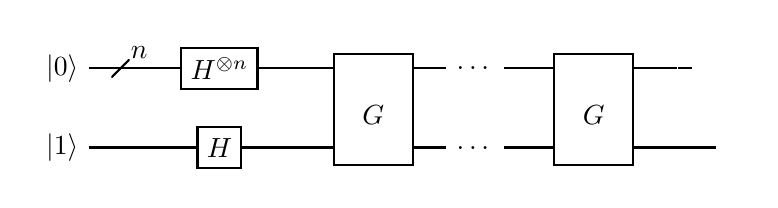
\begin{tikzpicture}[thick,
    cross/.style={path picture={ 
      \draw[black]
      (path picture bounding box.south) -- (path picture bounding box.north);
    }},
    swap/.style={path picture={ 
      \draw[black]
       (path picture bounding box.south west) -- (path picture bounding box.north east) 
       (path picture bounding box.south east) -- (path picture bounding box.north west);
    }},
    bundle/.style={path picture={ 
      \draw[black]
      (path picture bounding box.south west) -- (path picture bounding box.north east);
    }}]

    % `operator' will only be used by most gates.
    % `cnot' will refer to CNOT gates.
    % `phase' is used for controlled gates.
    \tikzstyle{operator} = [draw,fill=white,minimum size=1.5em]
    \tikzstyle{cnot} = [draw,cross,circle,minimum size=5pt]
    \tikzstyle{meter} = [draw,color=white,fill=white,minimum size=1.7em]
    \tikzstyle{phase} = [draw,fill,shape=circle,minimum size=5pt,inner sep=0pt]
    %
    \matrix[row sep=0.4cm, column sep=0.8cm] (circuit) {

    % First row.
    \node (S0) {$|0\rangle$};&[-0.5cm] 
    \node[bundle] (B0) {}; 
    \node[above right] (B0) {$n$}; &[-0.5cm] 
    \node[operator] (O12) {$H^{\otimes n}$}; 
    &
    &
    & 
    \node (O14) {\ldots}; 
    &
    &
    &
    \node[meter] (M11) {\pgfbox[center,center]{\pgfuseimage{meter}}};
    \coordinate (end1);\\
    
    % Second row.
    \node (S1) {$|1\rangle$};&[-0.5cm] 
     &
     \node[operator] (O22) {$H$};& 
     &
     &
     \node (O24) {\ldots}; 
     &
     &
     &
    \coordinate (end2);\\
    };
    \draw [thick,black,fill=white] (-0.7,-2.2em) rectangle (0.3,1.8em);
    \node at (-0.2,-0.14) (O) {$G$};
    \draw [thick,black,fill=white] (2.1,-2.2em) rectangle (3.1,1.8em);
    \node at (2.6,-0.14) (O) {$G$};
    
    \begin{pgfonlayer}{background}
        % Draw lines.
        \draw[thick] (S0) -- (O14) (O14) -- (end1) (S1) -- (O24) (O24) -- (end2)
                     ;
    \end{pgfonlayer}
    %
    \end{tikzpicture}
\end{document}
